\documentclass[12pt,oneside]{book}
\usepackage{0protoposal}
%\setuptodonotes{disable}

\begin{document}
\begin{titlepage}\centering
    \begin{figure}[ht!]\centering
\includegraphics{bruni-logo.png}\end{figure}
    \vfill\textbf{\Huge Playing the Periphery}\vspace{24mm}\\
    {\huge A thesis submitted for the degree of\\MA Games Design\\
    \vspace{8mm}by}\vspace{8mm}\\\texttt{\LARGE 2\>4\>4\>1\>8\>7\>1}\vfill
    {\Large Department of Arts and Humanities, Brunel University London}
\end{titlepage}

\tableofcontents\begingroup\let\clearpage\relax\listoffigures\endgroup

\newgeometry{top=16mm,bottom=16mm}
\chapter*{Abstract}\addcontentsline{toc}{section}{Abstract}
  \begin{center}\begin{singlespace}
    My topic of interest lies at the intersection of paratextual, corporeal, and sociocultural aspects of iconic game titles and their impact of their legacy.
    In other words, elements that lie at and/or outside the perimeter of the magic circle\parencite{huizinga}.
    Paratext consists of surrounding media not included in the game itself but strongly influencing how the experience is accessed, framed, and understood.
    Material comprises the physical means and contexts of play, in turn shaping the experience through sensory input, physical feedback, and presence. 
    Community is embodied by the players themselves through shared habits, beliefs, and informal systems.
    The synergy of this trinity is flavoured by the aesthetics of the game playing experience in its entirety.
    Moreover, pairing any of these three permeates another facet of that external conceptual space.\par
    In consideration of these angles, my project poses the following question:
    \begin{displayquote}
        \textbf{\textit{In what ways can contemporary game design achieve holistic aesthetic experiences in the likeness of historically acclaimed game titles?}}
    \end{displayquote}
    The research perspective is mostly aimed at context awareness and experiential revision, although, nostalgia remains a latent yet potent factor that bears investigation.
    Retrospective settings are being highlighted because most well-known titles from the past represent history as written by the victors.\footnote{Or, in a few amusingly infamous cases, the kitschy underdogs and dark horses that are often both cautionary tales and subjects of cult following. Evidently, if one struggles to attain immortality via glory, becoming an anecdote remains a viable alternative.}
    With this in mind, I believe that game design can notably benefit from closely examining the external circumstances which frame any media product's release.\par
    The theoretical research will examine existing frameworks established in game and media fields of study, intending to touch on fields and concepts such as 
    experiential aesthetics, affect theory, procedural rhetoric, immersion, metagaming, preservation, and various design approaches.
    The practical review will survey an assortment of games whose play experience is notably characterised by contextual circumstances.
    This investigation is meant to derive patterns from exemplary case studies that can suggest ways of implanting the external layers of play experience into a new piece of playable media.
    With historical awareness providing the background, some of the findings will be incorporated into designing a digital artifact complementing the written one, accompanied by fictional context in the shape of lore and paraphernalia.\par
    Comprehensive analysis of multiple real world scenarios is to be followed by a selection of applicable
    \footnote{A word which here means \parencite{asoue} "feasible".}
    approaches, which in turn will inform the directions taken throughout the design and development process.
    Concurrently, any relevant observations should be recorded with the intent to feed back into the writing and, eventually, provide a strong basis for reflection.
    Exercising theory in practice is expected to direct the unfolding of the game's design.
    The goal that I aspire to achieve with this project is tracing a model of media creation that is elevated by its surrounding context, and also aligns with key values established in my personal game design philosophy \parencite*[GD5609,][]{myDesignPhil}, then put the resulting framework into future practice.
\end{singlespace}\end{center}
\restoregeometry\clearpage

\chapter{Introduction}
\section*{Extrinsic Circles}
Contextual influences and overall legacy impact are among the focal points for both primary and secondary sources considered in this paper.
Theoretical examinations will mostly engage with the humanities of game studies - particularly sociocultural and media fields.
    \todo[add]{One sentence summary of written sources}
However, the research question is more for the benefit of exploring an outside-in perspective on production and design, so it will be supported by practical use cases.
    \todo[add]{One sentence summary of gaming sources}
    \vfill
\begin{figure}[ht]
    \tikzperi\caption{Peripheral aspects of play}\label{peri-play}
\end{figure}
    \vfill
When put together, Paratextuality, Physicality, and Popularity can be treated like X/Y/Z dimensional axes. Given any game as a source, evaluating its properties as measures along these axes yields coordinates that denote the facets of paraphernalia, preservation, and personalisation.
\clearpage
\section*{Premise}
I have made the possibly unconventional choice of splitting the practical half of this project further into two games.
One has the digital prototype role, while the other is rather a conceptual case study.
The reason for that approach is a matter of positioning.
In order to focus on analysing the outer spaces of gameplay experience, it is almost imperative that the foundation itself is built \textit{outside} said gameplay, with the design \& creation process directed \textit{inwards}.
Keeping in mind the immutable reality of human limitations, a retrospective inquiry at the aesthetic legacy and sociocultural impact of a video game developed by a solo student, on a scale large enough to be of any consequence, is not only an infeasible undertaking, but one that would naturally steer all efforts towards actual development at the expense of design.
Although that would be an achievement of large proportions, it would bring little value towards the purpose of this exercise.
As it turns out, the subject of the case study does not, technically, exist.
At least not in the form of the playable media it is supposed to to represent.
Rather, it shall be defined through negative space, i.e., the silhouette made from all the shapes that are not intrinsic to its architecture.
Design will largely be catered by the lost game, while implementation will be relegated to the mini game.
The latter has the role of an interactive loading screen, serving as waiting distraction that provides some preparatory advice for the former.
Detailed overviews for both game layers can be found in Chapter \ref{chap-4-dev} and Appendix \ref{apdx:paratxt}.

\chapter{Literature Review}
    \todo[ref,inline]{Friedrich Adolf Kittler versus Marshall McLuhan \nocite{mcluhan} on media theory}
    \todo[ref]{Metagames\nocite{boluk-lemieux}}

\section{Paratextuality}  
    The initial concept by G\'{e}rard Genette \parencite*{genette} has been considerably expanded to better fit the field of game studies, and as a result has been entangled with adjacent terms from the original scholar's typology. \footnote{The five aspects of \textit{trans}textuality comprise of: \textit{inter}-, \textit{meta}-, \textit{hyper}-, \textit{archi}-, and \textit{para}-texts.}
    However, both approaches can be integrated into my own, owing to the generous overlap between the three types of external context.\par
    When strictly categorising cases, Genette's definition regards 
    ``Elements that form a figurative threshold of a text and ground it in a socio-historical context. [...] must be created by the text’s producers or their associates".
    These can be promotional materials, introductory sequences, menus, credits, making-ofs, contextual information about authors.\par
    While preserving Genette's wording on which elements are included, Consalvo's interpretation assigns ``...no limitations on authorship or cultural status" \parencite*{consalvo}. 
    This is akin to \textit{cultural epiphenomena} and allows consideration of more media like ``criticism and journalism, user discussions, fan fiction and fan art, streaming, trans-media storytelling" \parencite{svelch}.\par
    On these grounds, Genette's delineation is the more clear and straightforward directive for labelling purposes, while Consalvo's expansion on it draws a connection to cultural assimilation.
    Additionally, both have ties to materiality in their manifestation.
\section{Physicality}
        \todo[add]{proper lit review of \citetitle{bogost-platform} and \citetitle{kirschenbaum}}
    The most tangible of the three aspects, this refers to all the material conditions in which the game is played.
    Exclusively, this covers authentic hardware and peripherals, physical data storage, haptic features, and environmental settings.
    In addition, paratextual supplements in physical format, e.g., paper, fall under the same category to form paraphernalia.
\section{Popularity}
        \todo[add]{proper lit review of \citetitle{grimes}, \citetitle{taylor}, 
            \citetitle{gitelman}, \citetitle{hjenkins}, \citetitle{keogh}}
    Culture and society permeate the first two aspects via informal systems of shared habits, beliefs and conventions.
    The formation of social rituals by the demographic over time leads to emergent paratext, stemming from reception and circulation, and physical aspects are embodied in player presence and direct interaction with the hardware.

\chapter{Case Studies}
    \todo[add]{Curate primary sources\\
        \citetitle{ufo50}; \citetitle{inscryption2021};
        Feelies, Swordquest; Startropics; \citetitle{vectrex-bytemag};}
    \todo[ref,inline]{Support with secondary sources:
        \citebook{sicart-argo}, 
        plus zines and such like Your Sinclair, Commodore User, Compute!, Antic, etc.}
    \todo[add]{Apply P-framework}

\chapter{Development}\label{chap-4-dev}
    \todo[ref,inline]{Guidance from Deep Games by \cite{rusch}}

\section{The Lost AMOLED}
Clever Rebel Trials was an ambitious attempt to reinvent platform exclusivity following the 4th Generation's Console Wars.
Rather than developing a killer app for a designated system, Adelin Melony (1970-2002) set out to create a machine whose sole purpose was to play the one game that it was optimised for.
The game itself was released in 1997 on the Ludic Entertainment Device - its dedicated Generation 4.5 console that was soon dubbed ``Addie Mel's One-Shot LED', shortened to AMOLED.
While the approach is not unheard of (being a standard practice for arcade acabinets and many 1st and 2nd generation products) such an idea carries major risks concerning scope, audience demand and reception.

CRT is set in a retro-futuristic world with competing factions offering exclusive membership perks.
The main gameplay loop revolves around managing a multitude of characters from the Clever Rebels Team.
Each rebel specialises in a very narrow field of studies, which makes for entirely different character builds and run strategies.

\paragraph{Notes from the GM}
The creator's names are anagrams using the first names of Daniel Handler, whom she also shares a birthday with, and his pseudonym Lemony Snicket. Chronologically, her lifetime closely matches the birth and growth of videogame technology, but was sadly cut short when she was only 32 years old.\par
Although they have been swapped and scrambled into vague equivalents, most names within this alternate universe originate from the ASOUE books \parencite{asoue}.\par
In them, there are also mentions of a secret organisation called VFD. In Snicket's world VFD stands for Volunteer Fire Department, but in ours, among other things, it means Vacuum Fluorescent Display. I found the notion of using other display type acronyms amusing, hence CRT and LED/AMOLED.\par
Beside having a name reminiscent of NES, the LED console with its CRT game came out at a time of a literal dimensional shift in computer graphics technology - a transition from 16-bit pixels on cartridges to 32-bit polygons on optical discs with all the new rendering and memory management methodologies it brought about.
\footnote{It also may or may not conveniently share a birthyear with yours truly.}

\section{Prototype}
    \todo[ref,inline]{Primary sources for direction: 
        \\ Space Invaders loading mini-game and The Sims cases}
    \todo[rtd]{Layout \& UI:
        \\\hspace{8mm}screens correspond to hand placement: left hand collects water, right hand steers the truck
        \\\hspace{8mm}controls were "canonically" separate dials (and/or even meant for two players?)
        \\\hspace{8mm}here they are tied to a single mouse which is why each is confined to a single axis
        \\\hspace{8mm}loading bar tracks the mini-game's progress under the hood
        \\\hspace{8mm}maybe our goal can be to have the player ignore the launch button once it appears
        \\\hspace{8mm}tips give ambiguous clues for the main game; juicier details come later on}
    \todo[rtd]{Environment:
        \\\hspace{8mm}Trees at varied grown stages spawn over time. The bigger the tree:
            \\\hspace{16mm}the more likely it is to spawn small trees around itself
            \\\hspace{16mm}the more flammable it is, but generates larger clouds
        \\\hspace{8mm}Raindrops fall at the same speed but appear faster from larger clouds
        \\\hspace{8mm}right now mouse buttons serve as pedals for the fire truck
        \\\hspace{8mm}already seems a bit tricky to multitask, I may automate movement
        \\\hspace{8mm}truck and bucket upgrades for successful fire management}
            
% ASSETS AND ALL%
\citetitle{kenney-1bit}; \citetitle{font-adore64}; \citetitle{crt-shader}
    \todo[dev,noinline]{ASSET HUNT:
        background?,
        cursor?,
        loading bar,
        steering wheel,
        sounds and animation}

\begin{figure}[ht!]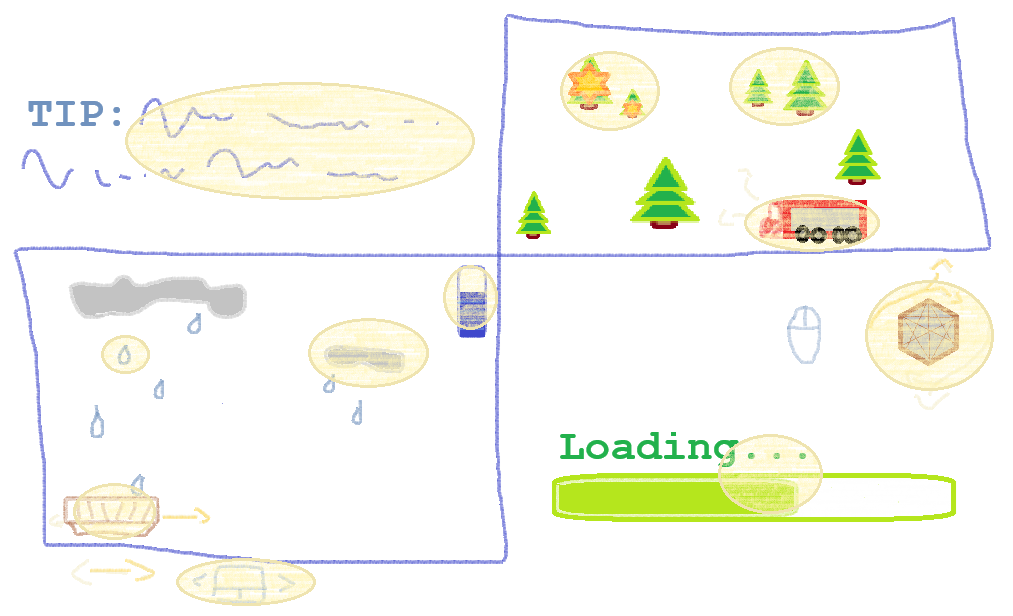
\includegraphics[width=0.8\textwidth]{MA-idea.png}
    \centering\caption{``Paper'' prototype}\label{paper-proto}
\end{figure}
    \todo[app,noinline]{wireframe with legit software}

    \todo[dev]{opening screen}
    \todo[dev]{tree growth stages}
    \todo[dev]{fully grown trees $\to$ saplings}
    \todo[dev]{forest coverage $\to$ cloud size}
    \todo[dev]{cloud size $\to$ raindrops amount}
    \todo[dev]{correct car controls}
    \todo[dev]{auto-pilot fire-truck}
    \todo[dev]{upgradable bucket}
    \todo[dev]{auto-collecting bucket}
    \todo[dev]{score $\to$ loading progress -> full bar $\to$ start button to end game}

\section{Periphery}
    \todo[ref,inline]{Primary sources for direction: 
        \\ Final Fantasy jobs and Children of Morta for skill progression
        \\ Magnavox Odyssey and Vectrex for odd hardware}

\subsection*{Paraphernalia}\hfill\textit{Paratextuality + Physicality}
    \todo[add]{Manual and machine}

\subsection*{Preservation}\hfill\textit{Physicality + Popularity}
    \todo[add]{What has survived, in what format, and why?}
    \todo[add]{Hardware quirks: dials, 2 screens?}

\subsection*{Personalisation}\hfill\textit{Paratextuality + Popularity}
    \todo[add]{Interpretations and practices shaping legacy = discussion + review}

\section{Product}
    \todo[add]{Why does the mini-game exist? (fic)
        Calibration for both platform and player
        Check controls work propery while getting used to the game overall}
    
\chapter{Synthesis}
    \todo[add]{Theory in practice: how they informed and/or clashed with each other}
    \todo[add]{Revision of the artifact(s)}
    \todo[ref,inline]{Correlation with sources?}
    \todo[add]{Provisional answer to the research question.}

\chapter{Conclusion}
    \todo[add]{Critical reflection on achievement}
    \todo[add]{Outline of implications and further research directions to build upon.}
    \todo[ref,inline]{Recommended reading/playing not mentioned in earlier chapters}
\vfill
    \todo[add]{\Large Final word count minus references, footnotes and appendices}
    %     456 Abstract
    %    +370   out of  400 exp. in Chapter 1
    %    +290   out of 2400 exp. in Chapter 2
    %           out of 1800 exp. in Chapter 3
    %    +320   out of 1400 exp. in Chapter 4
    %           out of 1600 exp. in Chapter 5
    %           out of  400 exp. in Chapter 6
\hfill\textit{\large Word count: 1436}
\newpage\addcontentsline{toc}{chapter}{References}
\printbibliography[title={\LARGE Bibliography}, filter=readings]
\printbibliography[title={\LARGE Ludography},   type = software]
\printbibliography[title={\LARGE Assets},       filter = assets]

\newpage\newgeometry{margin=4mm}
\titleformat{\chapter}[hang]{\bfseries\LARGE\scshape}{
    Appendix \thechapter}{32ex}{} \appendix
\chapter{Paratexts}                        \label{apdx:paratxt}
\section{Manual}                           \label{apdx:manual}
    \todo[app]{Setting and Campaigns}
    \todo[gpt]{Key factions and events; Known unknowns
            \\\hspace{8mm}Events everyone references but noone explains fully
            \\\hspace{8mm}Past figures whose actions shape the present
            \\\hspace{8mm}Conflicting records}
    \todo[app]{Characters' Progression \& Skill trees}
    \todo[app]{Hardware notes}
\newpage\section{Articles}
\subsection*{A.2.1 \quad Magazine preview} \label{apdx:mag-art}
    \todo[app]{Write promo content}
\begin{figure}[h!]\centering
    \includegraphics[page=2, scale=0.64, angle=-90]{para-mag.pdf}
    \vspace{-16mm}\\
    \includegraphics[page=3, scale=0.64, angle=-90]{para-mag.pdf}
\end{figure}\clearpage
\subsection*{A.2.2 \quad Webpage review}   \label{apdx:web-art}
    \todo[app]{Scaffold HTML page}
    \todo[app]{Write critical content}
\section{Message board(s)}                 \label{apdx:msg-thr}
    \todo[app]{Scaffold HTML page}
    \todo[app]{fill thread with user comments}

\newpage\listoftodos
\end{document}